\chapter{Group Homomorphism and Isomorphism}\label{chp:1_8}

\begin{definition}{}{}
    Let $G$ and $H$ be semigroups.
    A function $f:G\rightarrow H$ is a homomorphism
    if $f(ab)=f(a)f(b)$ for all $a,b\in G$.
    A one to one (injective) homomorphism is a monomorphism.
    An onto (surjective) homomorphism is an epimorphism.
    A one to one and onto (bijective) homomorphism is an isomorphism.
    If there is an isomorphism from $G$ to $H$, we say that
    $G$ and $H$ are isomorphic, denoted $G\cong H$. 
    A homomorphism $f:G\rightarrow G$ is an endomorphism of $G$.
    An isomorphism $f:G\rightarrow G$ is an automorphism of $G$. 
\end{definition}

\begin{proposition}{}{}
    If $f : G \rightarrow H$ and 
    $g : H \rightarrow K$ 
    are homomorphisms on semigroups $G, H, K$,
    then the composition $g \circ f = gf : G \rightarrow K$ 
    is a homomorphism. 
    Similarly, compositions of monomorphisms, epimorphisms, isomorphisms, and automorphisms are
    respectively monomorphisms, epimorphisms, isomorphisms, and automorphisms.
\end{proposition}

\begin{proposition}{}{}
    a group homomorphism maps identities to identities and inverses to inverses.
\end{proposition}

\begin{definition}{}{}
    Let $f:G\rightarrow H$ be a homomorphism of groups.
    The kernel of $f$ is $\text{Ker}(f)=\{g\in G:f(g)=e_H\in H\}$.
    If $A\subset G$, then the image of $A$ is $f(A)=\{h\in H:h=f(a) \text{ for some }a\in A\}$.
    The set $f(G)$ is called the image of homomorphism $f$, denoted $\text{Im}(f)$.
\end{definition}

\begin{proposition}{}{}
    Let $f:G\rightarrow H$ be a homomorphism of groups. Then:\\
    (1) $f$ is a monomorphism if and only if $\text{Ker}(f)=\{e_G\}$;\\
    (2) $f$ is an isomorphism if and only if there is a homomorphism
    $f^{-1}:H\rightarrow G$ such that $ff^{-1}=1_H$ and $f^{-1}f=1_G$.
\end{proposition}


\begin{theorem}{}{canonical epimorphism thm}
    If $f:G\rightarrow H$ is a homomorphism of groups,
    then the kernel of $f$ is a normal subgroup of $G$. Conversely,
    if $N$ is a normal subgroup of $G$,
    then the map $\pi: G\rightarrow G/N$ given by $\pi(a)=aN$ is an epimorphism
    (that is, an onto homomorphism) with kernel $N$.
\end{theorem}

\begin{definition}{}{}
    The map $\pi:G\rightarrow G/N$ of theorem \ref{thm:canonical epimorphism thm}
    defined as $\pi(a)=aN$ is the canonical epimorphism.
\end{definition}

\begin{theorem}{}{}
    If $f : G \rightarrow H$ 
    is a homomorphism of groups, 
    then $f$ induces an isomorphism of
    $G/\text{Ker}(f)$ with $\text{Im}(f)$. 
\end{theorem}

\begin{figure}[H]
    \centering
    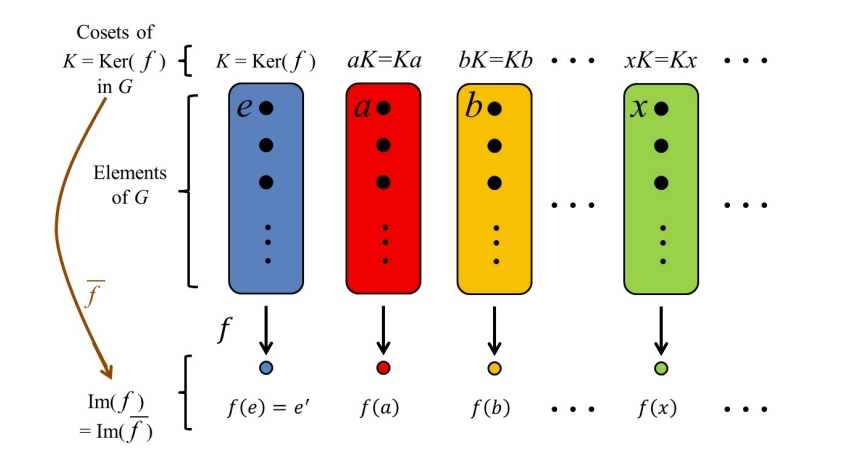
\includegraphics[width=0.6\textwidth]{figure/isomorphism.png}
    \caption{}
\end{figure}

\section{Reference}

\begin{itemize}
    \item \href{https://faculty.etsu.edu/gardnerr/5410/notes/I-2.pdf}{Homomorphisms}
    \item \href{https://faculty.etsu.edu/gardnerr/5410/notes/I-5.pdf}{Homomorphisms}
\end{itemize}

